\chapter{Background}
	
	This chapter gives an overview of the problems involved in the simulation of
	brains followed by a brief survey of current super computer technology and the
	challenges it faces. This is followed by a summary of the leading
	special-purpose neuromorphic architectures being developed to tackle the
	shortcomings of modern supercomputers. The chapter concludes with a detailed
	exploration of the SpiNNaker platform and the interconnection technology it
	uses which form the basis of my research.
	
	\section{Simulating brains}
		\label{sec:simulating-brains}
		
		% What is done, for what purpose
		
		The brain is an extremely complex and variable organ whose high-level
		behaviours are similarly complex and variable. Efforts to understand the
		brain, unsurprisingly, rely on simplified models of its function. This
		section gives a brief history of the development of artificial neural
		networks leading to an outline of the models used today. This is followed by
		a description of the general structure and behaviour of simulators for such
		models and the computational challenges this entails.
		
		\subsection{History of artificial neural networks}
			
			The development of ANNs can be divided up into three coarse generations,
			each increasing their level of biological realism \cite{vainbrand11}.
			
			The first generation of ANNs, such as the McCulloch-Pitts threshold neuron
			\cite{mcculloch43}, consisted of testing if a simple, linear function of
			the neuron's inputs was above a threshold value and outputting either a
			`high' or `low' signal. The function used in each neuron and the pattern
			of connectivity in the network define the behaviour of the network as a
			whole.
			
			It was realised that communication between neurons is not level-based but
			instead appears to be based on the rate at which `spikes' are produced (or
			`fired') by neurons to their neighbours. The second generation of ANNs
			seek to model this by representing the `firing rate' as their output in a
			continuous value \cite{maass97}. Once again, the network's behaviour was
			defined by the functions computed by each neuron and the network's
			connectivity.
			
			\begin{figure}
				\center
				\input{|"python2 figures/snn-example.py"}
				\caption{Simple leaky-integrate-and-fire neuron example.}
				\label{fig:snn-example}
			\end{figure}
			
			The third generation of ANNs extends the idea further by realising that
			the firing rate is not the only significant factor but that the timing of
			the arrival of spikes is significant too \cite{maass01}. In addition, many
			of these models aim to reproduce observed physiological behaviours of
			individual neurons, rather than simply recreate higher-level behaviours of
			populations of neurons. The level of biological detail of such models
			varies greatly but all tend to build on the `leaky integrate and fire'
			model.
			
			Spikes arriving at a neuron cause ion channels to open temporarily
			allowing a flow of current in or out of the neuron. The neuron integrates
			the current over time, accumulating charge which gradually leaks away over
			time. If the charge in the neuron reaches a certain threshold, it produces
			a spike and its charge is reset. This process is illustrated in figure
			\ref{fig:snn-example}.
		
		\subsection{Learning}
			
			In addition to the basic spiking behaviours exhibited by neurons, the
			mechanism by which they learn is also the subject of much research.
			Learning models in spiking neural networks largely revolve around
			adjusting the `weights' associated with connections between neurons based
			on the relative timing \cite{pfister06} or rate \cite{bienenstock82} of
			spike arrivals at a neuron. These weights control the amount of current
			that flows into a neuron when a spike arrives and thus the impact it may
			have on the neuron's spiking behaviour. Some learning rules can also form
			entirely new connections between previously disconnected neurons,
			essentially assigning a weight non-zero to the connection
			\cite{bamford10}.
		
		\subsection{Computation}
			
			Computationally, spiking neural models can be relatively simple, the state
			of the neuron is described by a differential equation over time. Neuron
			states are typically updated with a fairly coarse granularity of once per
			0.1 to 1.0 ms. Additional calculations are also required to update the
			neurons' states upon spike arrival. In the case of networks featuring
			learning models, spike arrivals also typically entail further calculations
			in order to update weights.
			
			Given that biological systems may contain billions of neurons and
			trillions of synapses spiking at an average rate of 10 Hz, this
			constitutes a non-trivial amount of of computation even for the simplest
			models. In order to maintain real-time performance, the simulation of
			different neurons must be distributed across a large number of processing
			cores.
		
		\subsection{Communication}
			
			% Number of spikes produced, the form that spikes take, multicast,
			% possible changes due to learning. Especially fun for real-time.
			
			The feature of neural models which stresses simulators most, however, is
			their communications requirements. Each neuron in biologically realistic
			systems may be connected to around 10,000 other neurons. In distributed
			systems, this means that each spike may need to be transmitted to a large
			number of destinations. Conventional computer networks tend to be focused
			on supporting efficient one-to-one connectivity. In many cases this means
			that each spike must be repeatedly sent, once to each destination, which
			costs both large amounts of network resource and also power. To achieve
			greater efficiency, multicast communications can be used where the message
			is sent once and is delivered to multiple locations.
			
			An additional challenge for interconnection models is the granularity of
			communications in neural simulators. Spike messages encode only a very
			limited amount of data: their source neuron and the time they were
			produced. This means that individual messages sent through the network
			tend to be very small even though the aggregate network utilisation may be
			high. This pattern is directly opposed by conventional computational
			problems which instead tend to transmit large, continuous blocks of data
			at infrequent intervals. As a result, conventional networks can impose
			large overheads when dealing with spikes.
			
			Luckily, much of the connectivity within the brain is highly local meaning
			that neurons tend to mostly connect to physically nearby neurons. This
			type of predominantly local communication is well supported by most
			scalable computer networks such as those found in supercomputers. In order
			to take advantage of this property, however, neural models must be
			carefully laid out within a simulator's network. This problem known to be
			NP-complete though highly performant heuristic solutions have been
			developed for use in other fields such as VLSI and FPGA design
			\cite{haldar00}.
	
	
	\section{Supercomputer technology}
		\label{sec:supercomputers}
		
		\begin{table}
			\center
			\begin{tabular}{r l r r r l l l}
				\toprule
				Rank & Name    & Pflops& Cores  & Nodes  & Topology & Interconnect          & Sources \\
				\midrule                          
				1 & Tianhe-2   & 33.86 & 3,120,000 & 16,000 & Fat-Tree & Electrical \& Optical & \cite{dongarra13} \\
				2 & Titan      & 17.59 & 560,640   & 18,688 & 3D Torus & Electrical            & \cite{bland12} \\
				3 & Sequoia    & 17.17 & 1,572,864 & 98,304 & 5D Torus & Electrical \& Optical & \cite{prickett10} \\
				4 & K Computer & 10.51 & 705,024   & 68,544 & 6D Torus & Electrical            & \cite{fujitsu11,yokokawa11} \\
				5 & Mira       &  8.59 & 786,432   & 49,152 & 5D Torus & Electrical \& Optical & \cite{prickett10} \\
				\bottomrule
			\end{tabular}
			
			\caption{Top Five `Top500' Super-Computers, November 2013 \cite{meuer13n}.}
			\label{tab:top500}
		\end{table}
		
		The Top500 list \cite{meuer13n} aims to enumerate, biannually, the 500
		fastest super-computers ranked by their performance on the LINPACK benchmark
		\cite{dongarraLINPAC}. The list offers an insight into the current
		state-of-the-art for high-performance computing. Table \ref{tab:top500}
		shows the top five machines in the Top500 list released in November 2013
		along with basic details of the type of interconnection involved. In this
		section an overview is given of the architecture of these large scale
		machines.
		
		The LINPACK benchmark performs computations to ``analyze and solve linear
		equations and linear least-squares problems'' to produce a computational
		load representative of certain computational tasks common to scientific
		computing \cite{dongarra84}. In particular it is a CPU-bound problem which
		attempts to measure the peak CPU performance achievable\footnote{Where CPU
		Performance is measured in Petaflops: how many quadrillion ($10^{15}$)
		floating point operations can be performed per second.} but without any
		significant indication of the performance of the network which connects the
		system together \cite{dongarra07}.
		
		Since simulation of spiking neural networks requires a large amount of
		communication but relatively small amounts of computation, this benchmark is
		clearly not representative of the workload of such a task.  In fact, many
		modern super-computer workloads also rely on network performance to a
		greater degree than the LINPACK benchmarks and as a result a new ranking,
		Graph500 \cite{murphy13n}, has appeared to address this shortcoming. This
		complementary ranking instead uses benchmarks based on graph traversal
		problems \cite{murphy10}. Such problems rely on having efficient
		point-to-point communication between different parts of the system where
		each section of the graph resides. Since there is a high degree of
		correlation between the rankings of the two lists, we just consider the more
		comprehensive Top500 list.
		
		
		\subsection{Anatomy}
			
			% What is in a typical super computer. Lots of CPU/GPU/Accel nodes with
			% comparatively limited interconnect. Vast amounts spent on power, cooling
			% etc.
			
			Supercomputers are typically built by combining a large number of
			`processing elements' in such a way that they are able to coherently
			perform a single task. The processing elements used can come in many forms
			though the three most prevalent are:
			
			\begin{description}
				
				\item[General Purpose Processor] A conventional processor `core' as
				found in desktop and mobile computer CPUs. These flexible devices have
				historically represented the vast majority of the Top500's computing
				power.
				
				\item[Graphics Processing Unit (GPU)] A specialised processor which is
				able to efficiently perform the same operation across a large number of
				data elements simultaneously (a technique called vector processing). The
				Titan super-computer notably makes extensive use of GPUs \cite{bland12}
				and these are growing in popularity in high-end super computers.
				
				\item[Accelerators] Increasingly other forms of more specialised compute
				resource, such as the Intel Xeon Phi accelerator used in Tianhe-2, are
				being used. The Xeon Phi contains 57 medium-sized general purpose cores
				which can be used to complement a conventional multi-core system
				\cite{dongarra13}. Other popular alternatives include FPGAs which can be
				reprogrammed to efficiently implement specialised algorithms in
				hardware.
				
			\end{description}
			
			A number of these individual processing elements are then combined
			together to create a single `node' in the system. This may take the form
			of an individual chip or a single circuit board. Typically the elements
			within a node are able to communicate relatively cheaply while messages to
			remote nodes must traverse a slower system-wide interconnection network.
		
		\subsection{Interconnect}
			
			In this subsection, the general structure and function of super computer
			interconnection networks is described, beginning with details of the
			high-level structure of the system and moving towards the low-level
			functions of the routers and link technologies used.
			
			\subsubsection{Topology}
				
				% Topology has influence on structure of the system, super computers are
				% optimised for local access of data near by. Two topologies are
				% popular: trees and tori.
				%
				% Trees have low hop counts and expensive routers, tori have higher hop
				% counts and cheaper routers. Both are easily partitioned.
				
				The topology of a supercomputer's interconnection network dictates the
				physical connections required to build it and constrains the patterns of
				communication the system can efficiently support. Topologies are
				typically designed such that communication between near-by nodes is
				cheap and does not compete with distant nodes for communication
				resources. The top five machines in the Top500 list achieve this using
				the `fat tree' and `torus' topologies which are described below:
				
				\begin{figure}
					\begin{subfigure}[t]{\textwidth}
						\center
						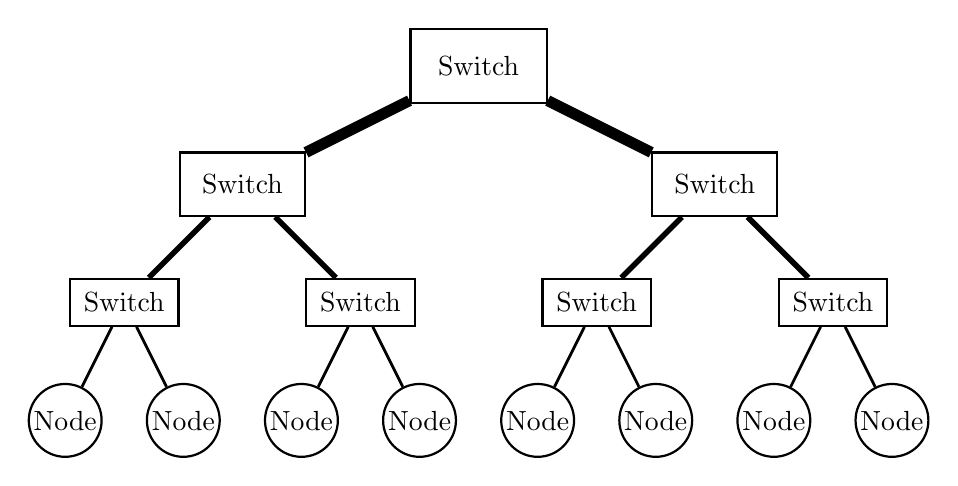
\begin{tikzpicture}[thick, node distance=1em]
	
	\begin{scope}[every node/.style={draw,rectangle,thick},inner sep=1.0em]
		\tikzstyle{level 1}=[sibling distance=6cm,every child/.style  ={line width=4pt},inner sep=0.8em]
		\tikzstyle{level 2}=[sibling distance=3cm,every child/.style  ={line width=2pt},inner sep=0.5em]
		\tikzstyle{level 3}=[sibling distance=1.5cm,every child/.style={line width=1pt},inner sep=0.1em]
		
		\node {Switch}
			child {node {Switch}
				child {node {Switch}
					child {node [circle] {Node}}
					child {node [circle] {Node}}
				}
				child {node {Switch}
					child {node [circle] {Node}}
					child {node [circle] {Node}}
				}
			}
			child {node {Switch}
				child {node {Switch}
					child {node [circle] {Node}}
					child {node [circle] {Node}}
				}
				child {node {Switch}
					child {node [circle] {Node}}
					child {node [circle] {Node}}
				}
			}
		;
	\end{scope}
	
\end{tikzpicture}

						\caption{Basic fat tree links.}
						\label{fig:fat-tree-concept}
					\end{subfigure}
					
					\vspace{1.5em}
					
					\begin{subfigure}[t]{\textwidth}
						\center
						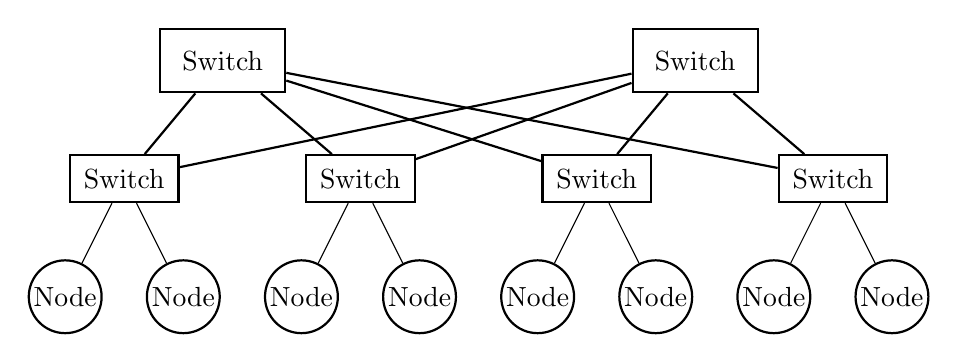
\begin{tikzpicture}[thick, node distance=1em]
	
	% Level 1 switches
	\foreach \n in {0,...,1}{
		\node (level 1 \n) at (2.0cm + \n*4*1.5cm,3.0) [draw,rectangle,inner sep=0.8em] {Switch};
	}
	
	% Level 2 switches
	\foreach \n in {0,...,3}{
		\node (level 2 \n) at (0.75cm + \n*2*1.5cm,1.5) [draw,rectangle,inner sep=0.5em] {Switch};
		
		\draw [thick] (level 2 \n) to (level 1 0);
		\draw [thick] (level 2 \n) to (level 1 1);
	}
	
	% Nodes
	\foreach \n in {0,...,7}{
		\node (node \n) at (\n*1.5cm,0) [draw,circle,inner sep=0.1em] {Node};
		
		\pgfmathtruncatemacro{\switch}{\n/2}
		\draw [thin] (node \n) to (level 2 \switch);
	}
	
\end{tikzpicture}

						\caption{Folded Clos network.}
						\label{fig:fat-tree-closs}
					\end{subfigure}
					
					\caption[Fat tree topologies.]{Fat tree topologies. Thicker lines
					represent higher bandwidth links.}
					\label{fig:fat-tree}
				\end{figure}
			
				In a basic fat tree, nodes are connected as leaves in a tree structure
				of multiple layers of switches (figure \ref{fig:fat-tree-concept}).
				Connections higher in the hierarchy are connected via links of
				increasing bandwidth to avoid bandwidth bottle-necks.  Nodes communicate
				by sending messages up the tree until it reaches a node with its
				destination as a child.
				
				In practice, as in `Tianhe-2', it is not possible to build switches with
				the required bandwidth. In addition, the root switch is a potential
				single point of failure for the whole system. As a result, folded Clos
				networks are often used instead (figure \ref{fig:fat-tree-closs}) and
				have become synonymous with the fat tree topology. Here higher levels of
				the hierarchy are duplicated introducing redundancy and spreading the
				load.
				
				Fat trees support small maximum `hop' counts, that is the number of hops
				a message has to make between nodes in the network. Specifically,
				average hop counts grow in fat trees by $O(\log{N})$ with respect to the
				number of nodes in the system. Additionally, they support cheap
				communication between nodes nearby in the tree.
				
				Unfortunately, tree-based networks depend on complex high-radix switches
				to connect many nodes simultaneously.  Tianhe-2, for example, has
				thirteen 576-port switches based on a custom router chip. Such
				architectures additionally often prove difficult to extend once
				implemented \cite{dally04}.
				
				\begin{figure}
					\begin{subfigure}[t]{\textwidth}
						\center
						\begin{tikzpicture}[thick,inner sep=0.1cm,3d/perspective eye={0,10,20}]
	\def\width{9}
	\def\height{9}
	
	\def\tubewidth{1}
	\def\holesize{5}
	
	\pgfmathtruncatemacro{\widthh}{\width - 1}
	\pgfmathtruncatemacro{\heightt}{\height - 1}
	
	\clip (-0.7,-0.3) rectangle (\widthh+0.7,\heightt+0.7);
	
	\foreach \lx in {0,...,\widthh}{
		\foreach \ly in {0,...,\heightt}{
			\node [fill,circle]
			      (node X\lx Y\ly) at (\lx, \ly)
			      {};
		}
	}
	
	% Draw normal links
	\foreach \x in {0,...,\widthh}{
		\foreach \y in {0,...,\heightt}{
			\pgfmathtruncatemacro{\xx}{\x + 1}
			\pgfmathtruncatemacro{\yy}{\y + 1}
			\ifthenelse{\xx < \width}{
				\draw (node X\x Y\y.center) -- (node X\xx Y\y.center);
			}{
				%\draw (node X\x Y\y.center) -- (node X0Y\y.center);
			}
			\ifthenelse{\yy < \height}{
				\draw (node X\x Y\y.center) -- (node X\x Y\yy.center);
			}{
				%\draw (node X\x Y\y.center) -- (node X\x Y0.center);
			}
		}
	}
	
	% Draw Long Links
	\begin{pgfonlayer}{background}
		\foreach \x in {0,...,\widthh}{
			\draw [help lines] (node X\x Y0.center)
			            .. controls +(0.7,-2.0)
			                    and +(0.7,2.0)
			            .. (node X\x Y\heightt.center);
		}
		\foreach \y in {0,...,\heightt}{
			\draw [help lines] (node X0Y\y.center)
			            .. controls +(-2.0,0.7)
			                    and +(2.0,0.7)
			            .. (node X\widthh Y\y.center);
		}
	\end{pgfonlayer}
	
\end{tikzpicture}

						\caption{Mesh (Grey lines show wrap-around connections added in a
						torus)}
						\label{fig:torus-flat}
					\end{subfigure}
					
					\vspace{1em}
					
					\begin{subfigure}[t]{\textwidth}
						\center
						\begin{tikzpicture}[thick,inner sep=0.1cm,3d/perspective eye={0,10,20}]
	\def\width{9}
	\def\height{9}
	
	\def\tubewidth{1}
	\def\holesize{5}
	
	\pgfmathtruncatemacro{\widthh}{\width - 1}
	\pgfmathtruncatemacro{\heightt}{\height - 1}
	
	\foreach \lx in {0,...,\widthh}{
		\foreach \ly in {0,...,\heightt}{
			\def\x{0};
			\def\y{\tubewidth};
			\def\z{0};
			
			\pgfmathsetmacro{\rotx}{(\ly*360)/\height}
			\pgfmathsetmacro{\roty}{(\lx*360)/\width}
			
			% Rotate points about x-axis depending on \ly to roll into a tube
			\pgfmathsetmacro{\xx}{\x}
			\pgfmathsetmacro{\yy}{\y*cos(\rotx) - \z*sin(\rotx)}
			\pgfmathsetmacro{\zz}{\y*sin(\rotx) + \z*cos(\rotx)}
			
			% Shift points along x-axis to make a tube
			\pgfmathsetmacro{\xxx}{\lx - (\width / 2)}
			\pgfmathsetmacro{\yyy}{\yy}
			\pgfmathsetmacro{\zzz}{\zz}
			
			\node [fill,circle]
			      (node X\lx Y\ly) at (3d cs:\xxx, \yyy, \zzz)
			      {};
		}
	}
	
	% Draw normal links
	\foreach \x in {0,...,\widthh}{
		\foreach \y in {0,...,\heightt}{
			\pgfmathtruncatemacro{\xx}{\x + 1}
			\pgfmathtruncatemacro{\yy}{\y + 1}
			\ifthenelse{\xx < \width}{
				\draw (node X\x Y\y.center) -- (node X\xx Y\y.center);
			}{
				%\draw (node X\x Y\y.center) -- (node X0Y\y.center);
			}
			\ifthenelse{\yy < \height}{
				\draw (node X\x Y\y.center) -- (node X\x Y\yy.center);
			}{
				\draw (node X\x Y\y.center) -- (node X\x Y0.center);
			}
		}
	}
	
	% Draw Long Links
	%\foreach \x in {0,...,\widthh}{
	%	\draw [red] (node X\x Y0.center)
	%	            .. controls +(0.5,-1.0)
	%	                    and +(0.5,1.0)
	%	            .. (node X\x Y\heightt.center);
	%}
	%\foreach \y in {0,...,\heightt}{
	%	\draw [red] (node X0Y\y.center)
	%	            .. controls +(-1.0,0.5)
	%	                    and +(1.0,0.5)
	%	            .. (node X\widthh Y\y.center);
	%}
	
\end{tikzpicture}

						\caption{Rolled into a tube}
						\label{fig:torus-pipe}
					\end{subfigure}
					
					\vspace{1em}
					
					\begin{subfigure}[t]{\textwidth}
						\center
						\begin{tikzpicture}[thick,inner sep=0.1cm,3d/perspective eye={0,20,30}]
	\def\width{9}
	\def\height{9}
	
	\def\tubewidth{1}
	\def\holesize{3.5}
	
	\pgfmathtruncatemacro{\widthh}{\width - 1}
	\pgfmathtruncatemacro{\heightt}{\height - 1}
	
	\foreach \lx in {0,...,\widthh}{
		\foreach \ly in {0,...,\heightt}{
			\def\x{0};
			\def\y{\tubewidth};
			\def\z{0};
			
			\pgfmathsetmacro{\rotx}{(\ly*360)/\height}
			\pgfmathsetmacro{\roty}{(\lx*360)/\width}
			
			% Rotate points about x-axis depending on \ly to roll into a tube
			\pgfmathsetmacro{\xx}{\x}
			\pgfmathsetmacro{\yy}{\y*cos(\rotx) - \z*sin(\rotx)}
			\pgfmathsetmacro{\zz}{\y*sin(\rotx) + \z*cos(\rotx)}
			
			% Shift off axis
			\pgfmathsetmacro{\xxx}{\xx + 0}
			\pgfmathsetmacro{\yyy}{\yy + 0}
			\pgfmathsetmacro{\zzz}{\zz + \holesize}
			
			% Rotate points around y axis depending on \lx to form doughnut
			\pgfmathsetmacro{\xxxx}{(\zzz*sin(\roty)) + (\xxx*cos(\roty))}
			\pgfmathsetmacro{\yyyy}{\yyy}
			\pgfmathsetmacro{\zzzz}{(\zzz*cos(\roty)) - (\xxx*sin(\roty))}
			
			\node [fill,circle]
			      (node X\lx Y\ly) at (3d cs:\xxxx, \yyyy, \zzzz)
			      {};
		}
	}
	
	% Draw normal links
	\foreach \x in {0,...,\widthh}{
		\foreach \y in {0,...,\heightt}{
			\pgfmathtruncatemacro{\xx}{\x + 1}
			\pgfmathtruncatemacro{\yy}{\y + 1}
			\ifthenelse{\xx < \width}{
				\draw (node X\x Y\y.center) -- (node X\xx Y\y.center);
			}{
				\draw (node X\x Y\y.center) -- (node X0Y\y.center);
			}
			\ifthenelse{\yy < \height}{
				\draw (node X\x Y\y.center) -- (node X\x Y\yy.center);
			}{
				\draw (node X\x Y\y.center) -- (node X\x Y0.center);
			}
		}
	}
	
	% Draw Long Links
	%\foreach \x in {0,...,\widthh}{
	%	\draw [red] (node X\x Y0.center)
	%	            .. controls +(0.5,-1.0)
	%	                    and +(0.5,1.0)
	%	            .. (node X\x Y\heightt.center);
	%}
	%\foreach \y in {0,...,\heightt}{
	%	\draw [red] (node X0Y\y.center)
	%	            .. controls +(-1.0,0.5)
	%	                    and +(1.0,0.5)
	%	            .. (node X\widthh Y\y.center);
	%}
	
\end{tikzpicture}

						\caption{Bent into a torus}
						\label{fig:torus-3D}
					\end{subfigure}
					
					\caption{Transformation of a mesh into a torus.}
					\label{fig:forming-a-torus}
				\end{figure}
			
				The most common topology in the top-five is the torus (also known as a
				$k$-ary $n$-cube). Here, nodes are arranged in a $n$-dimensional mesh.
				Nodes at the extreme edges of the mesh are connected together to form a
				torus. A 2D example is given in figure \ref{fig:forming-a-torus} which
				when rolled up (figure \ref{fig:torus-flat}) and bent into a doughnut,
				or torus shape (figure \ref{fig:torus-3D}) gives the torus network its
				name.
				
				Each node is able to communicate directly with its immediate neighbours
				in each dimension, that is above, below, left and right in the 2D case.
				More distant nodes are able to communicate by forwarding messages via
				intermediate nodes.
				
				As in the fat tree, nearby nodes are cheap to reach however a greater
				number of hops is required in the worst case: in a torus $k$ nodes long
				in each of $n$ dimensions the worst case path length is $\frac{kn}{2}$
				\cite{dally04}.
				
				Switches in torus networks can be simpler meaning that the worst case
				performance of both types of network can be comparable (17 $\mu$s for a
				broadcast in Tianhe-2 and 9 $\mu$s in a Blue Gene/Q such as Sequoia
				\cite{dongarra13,morozov12}).
				
				The differences in performance between tori and trees depends strongly
				on the application, however. Work by Vainbrand and Ginosar
				\cite{vainbrand11} showed that for spiking neural networks torus
				networks are preferable to fat-trees.
			
			\subsubsection{Link technology}
				
				% Universally high-speed-serial over optical and electrical links.
				% Optical is expensive but good for long distances. Always-on and so the
				% pressure is on to keep links fully loaded.
				
				Interconnect in modern super computers is made up almost exclusively of
				high-speed serial links running over either electrical or optical
				connections.
				
				Electrical transmission technologies are generally much cheaper than
				optical for short distances and lower bandwidths. As a result
				connections between physically neighbouring nodes are almost universally
				connected via such links.  Optical links, however, are favoured by super
				computer designs between cabinets containing many individual nodes in
				systems such as Blue Gene/Q and Tianhe-2 \cite{dongarra13,prickett10}.
				These optical links are typically used to carry the equivalent of many
				electrical signals and side-step difficulties with driving long distance
				electrical connections.
				
				High-speed serial links, which are described in more detail in a later
				section, use a single, high-frequency signal which encodes both data and
				a clock signal. This has a side-effect that the link must be constantly
				powered on in order to maintain a lock on the clock.  Power-efficient
				use of the link therefore requires implies that either the link is
				heavily loaded or that traffic in the network tolerate long latencies of
				thousands of cycles during link power-up \cite{soteriou03}. For neural
				simulations, which are generally latency sensitive and produce difficult
				to predict network traffic, this may require careful tuning of link
				behaviour to achieve power good efficiency.
				
				% TODO: Describe power control options for neural things
			
			\subsubsection{Packet formatting}
				
				Super-computer networks are generally designed to handle the transfer of
				large bursts of data on the order of several kilobytes in length making
				use of technologies such as Message Passing Interface (MPI)
				\cite{mpiforum12}. Since every MPI message must contain a header
				describing, for example, the message's origin and purpose, longer
				messages keep the overall overhead introduced low.
				
				This pattern is repeated in the low-level link protocols used by
				supercomputers too.  For example, in the widely used InfiniBand
				high-speed serial interconnect technology, 120 bytes of metadata are
				added to each packet \cite{infinibandta08}. This metadata allows the
				system to perform important tasks such testing for, and retransmitting,
				corrupt packets, route packets to their correct destination and apply
				flow control. Each packet can contain up to 4,096 bytes of payload
				meaning the overhead can be as low as 2.8\% protocol overhead.
				
				This pattern of communication matches many super computer applications
				as is reflected by the prominence of array and matrix functions in
				parallel programming APIs such as MPI. Unfortunately, this is a poor
				match for neural simulations which transmit only a single 32-bit integer
				to communicate spikes. If such a spike were transmitted individually
				over an InfiniBand link, the metadata would make up 96.8\% of the packet
				wasting significant bandwidth and energy.
				
				% TODO: Talk about work done by Xilinx and others. (Maybe?)
	
	
	\section{Neuromorphic computing}
		
		% Hardware which mimics biological systems more directly, essentially
		% optimised computers for neural simulations.
		
		\subsection{Analogue and mixed-mode}
			
			% Using analogue rather than digital electronics to accelerate the
			% computation of the various functions involved. Analogue circuits can
			% directly implement the differential equations required, can be very
			% tricky to calibrate, also inherently fixed. Interconnects often tend to
			% be digital to simplify things.
			
			\subsubsection{BrainScaleS}
				
				% Whole silicon wafer: extremely fast, extremely low power. Rather hard
				% to calibrate. Fair amount of flexibility in neuron model.
				%
				% Two interconnection systems: L1 and L2. L1 is circuit switched mesh
				% for low-power, low-latency connections, but very inflexible. L2 uses
				% FPGAs to translate into 10 gigabit Ethernet or other links. More
				% flexible and allows some scaling. Spikes multicast.
				%
				% Difficult to scale.
			
			\subsubsection{Neurogrid}
				
				% Very simple neural model, many chips in a tree. Communications are
				% digital and certain neuron features, such as connection weights are
				% modelled using probabilistic delivery. Spikes are serialised for each
				% chip. Between chips a tree is used.
				%
				% TODO: Does it use multicast?
				% TODO: Find out more about interconnect here.
			
		\subsection{Digital}
			
			% Use digital implementations of neurons, typically optimised in some
			% fashion.
			
			\subsubsection{Bluehive}
				
				% FPGA based, custom high-speed-serial interconnect, same link tech as
				% super computers, 3D torus network. Spike duplicated for all
				% destinations.
			
			\subsubsection{SpiNNaker}
				
				% CPU based, custom asynchronous multicast interconnect but scaling up
				% with high-speed serial 2D hexagonal torus network.
	
	
	\section{SpiNNaker network architecture}
		\label{sec:spinnaker}
		
		% Greater detail intro to SpiNNaker since it will be the focus of this work
		%
		% Overview of system: cores, chips, boards, racks, cabinets. Network is
		% hexagonal torus with nodes being chips.
		
		\subsection{Routing \& multicast}
			
			% Packet types and sizes. Table based routing, generally, multicast
			% routing in SpiNNaker. Also describe the sort of fun which can be had
			% with multicast, mention power savings due to less hops. Mention router
			% simplicity, limitations, assumptions.
		
		\subsection{Link technologies}
			
			% Between and within chips use asynchronous links. Between boards this
			% would be impractical due to number of wires and performance over long
			% wires. Instead, high-speed serial via FPGAs is used. Minimal torus
			% construction.
	
	\section{High-Speed Serial (HSS)}
		\label{sec:high-speed-serial}
		
		% Technology now used by most super computers and high-speed comms tasks.
		% More complex than parallel but they scale up throughput better.
		
		\subsection{Eliminating skew}
			
			% Parallel vs Serial, problems with parallel.
		
		\subsection{Clock recovery}
			
			% Requires frequent transitions (e.g. using 8b/10b) even on idle line,
			% makes idling expensive.
		
		\subsection{Clock correction}
			
			% Requires buffering clock/correction to deal with clock differences.
		
		\subsection{Error recovery}
			
			% Must retransmit packets with errors. Requires buffers.
		
		\subsection{Flow control}
			
			% Now unlimited amounts of data can be sent so must have way of applying
			% back-pressure. Again, means more buffering and complexity.
